\subsection{Optical Character Recognition}

In den meisten Fällen erfolgt eine Eingabe über eine Tastatur, jedoch ist dies manchmal weder die beste noch effizienteste Art, Text einzulesen. Mithilfe von \gls{ocr} ist ein automatisiertes Einlesen und Verarbeiten von handschriftlichen oder gedruckten Text möglich und das schon bereits in den 1950er. Am Anfang noch um Verkaufsberichte in Lochkarten zu konvertieren, damit ein Computer mit den Verkaufsdaten arbeiten kann \cite{OCR:online}.

Im Bereich von \gls{ocr} sind bereits momentan gute und präzise Resultate mit \glsfirst{ml} erwartbar, jedoch wie bei allen anderen Problem ist es verbesserbar. Um einen großen Fortschritt zu erreichen, würde die Nutzung von Deep Learning verpflichtend sein, dies ist jedoch in den meisten Situationen nicht notwendig.

Die Präzision hängt von vielen Attributen ab, daher kann ein eingescannter Text viel besser verarbeitet werden, als ein in der Freien geschossenes Bild mit dem Fokus auf ein Straßenzeichen \cite{OCR2:online}.

\begin{itemize}
    \item Textdichte

          Es macht einen Unterschied wie viel Text sich auf einer Fläche oder einem Bild befindet, denn es ist in gewissen Situationen leichter Text auszulesen, wenn dieser nur spärlich vorkommt.
    \item Struktur

          Wenn man eine klare Struktur erkennt, zum Beispiel in Tabellen oder in Zeilen, kann man ein besseres Ergebnis erwarten, daher ist es auch wichtig, dass man vor dem Auslese-Prozess das übergebene Bild aufbereitet und als Beispiel die Rotation ändert.
    \item Schriftart

          Handgeschriebene Texte oder ''laute'' Schriftarten sind im Gegensatz zu einfachen und gedruckten viel komplizierter, da sie kaum strukturiert sind. Außerdem könnten Buchstaben Ähnlichkeiten aufweisen, was später zu Verwechslungen führen kann.
    \item Buchstaben

          Sprachen wie Arabisch, Chinesisch, Russisch oder Japanisch benutzen im Gegensatz zu Deutsch ein anderes Alphabet, dabei kann es zu ähnlichen Buchstaben und Vertauschungen kommen, daher sinkt die Präzision in Texten mit mehreren Sprachen. Dies kann auch der Fall sein, wenn mathematische Formeln vorkommen.

          \begin{table}[H]
              \centering
              \begin{tabular}{|l|l|}
                  \hline
                  Kyrillisches Alphabet        & Ähnelt dem Buchstaben im lateinischem Alphabet \\ \hline
                  \foreignlanguage{russian}{r} & p                                              \\ \hline
                  \foreignlanguage{russian}{V} & B                                              \\ \hline
                  \foreignlanguage{russian}{N} & H                                              \\ \hline
                  \foreignlanguage{russian}{U} & y                                              \\ \hline
                  \foreignlanguage{russian}{S} & C                                              \\ \hline
              \end{tabular}
              \caption{Ähnlichkeiten zwischen Buchstaben im Lateinischem und Kyrillischem Alphabet}
          \end{table}
    \item Platzierung

          Zentrierte Texte erlauben ein besseres Auslesen, als abgeschnittene oder verstreute Wörter.
\end{itemize}

Die Texterkennung ist generell in zwei Phasen aufgeteilt:

\begin{itemize}
    \item Text Detection
    \item Text Recognition
\end{itemize}

\subsubsection{Text detection} ist der Prozess, indem in einem Bild oder einer PDF erkannt wird, wo sich Text befindet. Beim Resultat handelt es sich um Bounding Boxen, diese schließen einen Textblock (Wort, Buchstabe oder Paragraph) ein, dabei werden die genauen Koordinaten der Eckpunkte zurückgegeben. Diese werden später genutzt, um zur Visualisierung Boxen auf dem Bild oder der PDF aufzuzeichnen. Dieser Prozess wird auch in der Objekterkennung genutzt.

\begin{figure}[H]
    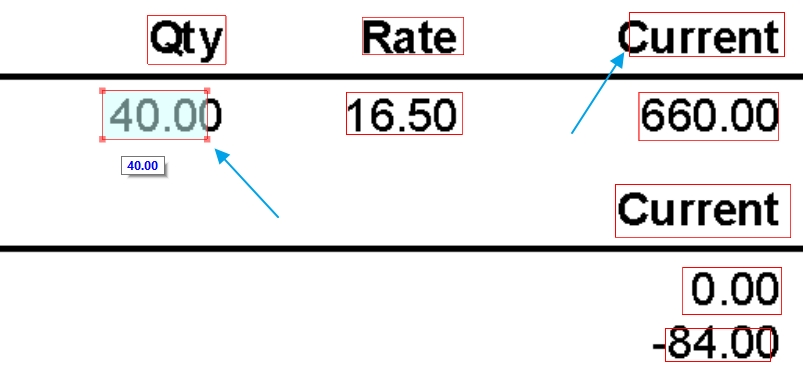
\includegraphics[scale=0.5]{sections/machine-learning/images/bounding-boxes.png}
    \caption{Bounding Boxes Beispiel}
    \label{fig:bounding-boxes}
\end{figure}

Die Erkennung kann entweder mittels der auf Regionen basierenden oder Textur basierenden Methode durchgeführt werden.

Bei der Regionen basierten Methode, werden Pixel verbunden und als Zeichenkandidat markiert, welche später mehrmals gruppiert werden und schlussendlich Wörter oder Textzeilen bilden. Dabei kommt es auf die geometrischen Eigenschaften an, wo es zu Fehlern beim Gruppieren kommen könnte. Wie man bei Abbildung \ref{fig:bounding-boxes} sehen kann, wurde der Buchstabe ''C'' im Wort ''Custom'' oder die letzte Nachkommastelle bei ''40.00'' nicht ganz als Teil des Wortes oder der Zahl erkannt.

Mit dem \Gls{swt} wird jedem Pixel eine Strichbreite zugeteilt, indem zwei Kanten gefunden werden mit der gleichen Richtung modulo 180°. Die Entfernung dieser zwei Kanten werden in den Kantenpixeln und alle unterliegenden Pixeln als Strichbreite gespeichert und alle Zusammenliegeden, gleich breite Pixel werden zu einem Zeichenkandidaten gruppiert. Danach werden alle benachbarten Zeichenkandidaten untersucht und zu einem Wort gruppiert, falls das mittelwertige Strichbreite-Verhältnis nicht über 2 liegt. Außerdem wird die Höhe und Farbe des Zeichenkandidaten berücksichtigt. Dies kann auch der Grund sein, wieso bei Abbildung \ref{fig:bounding-boxes} das Minuszeichen bei ''-84.00'' nicht zur Zahl hinzugefügt wird, das Minuszeichen ist signifikant niedriger als der Rest der Zahl. \cite{SWT:online}

\begin{figure}[H]
    \centering
    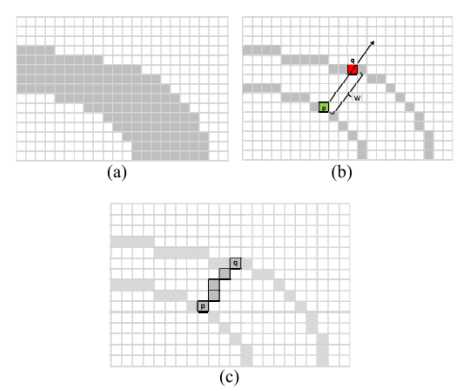
\includegraphics[scale=0.7]{sections/machine-learning/images/SWT.png}
    \caption{Die Kanten des Striches (a) werden solange verglichen, bis zwei gefunden werden mit der mit der gleichen Richtung (b). Alle unterliegenden Pixel erhalten die Strichbreite der Entfernung zwischen der Start- und Endkante (c).}
\end{figure}

Textur basierte Methoden unterteilen das Bild in Fester, dessen Höhe wird später mit der geschätzten Textgröße verglichen. Dabei kann es ebenfalls zu Erkennungsfehlern kommen.

Die Mischung dieser beiden Methoden gewann im Jahr 2011 den ICDAR-Wettbewerb mit einem F-Score von 71.28\%. Hierbei hat Chunghoon Kim den Vorschlag gegeben, dass als erstes Blöcke  mit dem \Gls{mser} Verfahren extrahiert und danach benachbarte Blöcke gruppiert werden, falls die Farbe und Größe sich ähnelt. Jedoch werden mit diesem Verfahren, ebenfalls eine große Menge an false-postive Blöcken erkannt. Um diese Anzahl zu verringern wird eine ähnlich Idee zur \gls{swt} verwendet. \cite{SWT:online}

\paragraph{Wettbewerbe}\label{ICDAR} sind ein großer Grund für die Fortschritte in der Texterkennung und im Rahmen des zwei-jährlich stattfindenden \Gls{icdar} Wettbewerbs wurden alle oben genannten Ideen verglichen \cite{ICDAR:online}.

\subsubsection{Text Recognition} ist genau wie bei der Erkennung von Text in zwei Möglichkeiten unterteilt: Regionen basierend und Textur basierend.

Die von \gls{mser} generierten und normalisierten Blöcke werden je nach der Orientierung in ein seerates Bild extrahiert. Dabei sind acht Orientierung möglich, welche mit ein Gaußschem Filter bearbeitet werden und auf ein 5 x 5 Bild komprimiert wurden. Mit diesen 5 x 5 x 8 = 200 dimensionalen Vektoren werden, dann die bereits erkannten Blöcke klassifiziert. \cite{SWT:online}
